\documentclass[a4paper,14pt,oneside,openany]{memoir}
\usepackage[left=30mm,right=15mm,top=20mm,bottom=20mm]{geometry}
\usepackage{polyglossia}
\setdefaultlanguage[indentfirst=true,forceheadingpunctuation=false]{russian}
\setotherlanguage{english}
\IfFontExistsTF{Times New Roman}
  {\setmainfont{Times New Roman}}
  {\IfFontExistsTF{FreeSerif}{\setmainfont{FreeSerif}}{\setmainfont{Liberation Serif}}}
\setmonofont{DejaVu Sans Mono}
\newfontfamily\cyrillicfonttt{DejaVu Sans Mono}[Script=Cyrillic]
\usepackage{indentfirst}
\usepackage{graphicx}
\usepackage{capt-of}
\usepackage{fancyvrb}
\parindent=1.25cm
\pagestyle{plain}
\renewcommand*{\chapterheadstart}{}
\renewcommand*{\printchaptername}{}
\renewcommand*{\chapnumfont}{\normalfont\bfseries}
\renewcommand*{\afterchapternum}{\hspace{1em}}
\renewcommand*{\printchaptertitle}{\normalfont\bfseries\centering\MakeUppercase}
\captionnamefont{\small}
\captiontitlefont{\small}
\captiondelim{ --- }
\counterwithout{figure}{chapter}
\setlength{\emergencystretch}{1.5em}
\begin{document}
\renewcommand{\figurename}{Рисунок}
\thispagestyle{empty}
\begin{center}
МИНИСТЕРСТВО ЦИФРОВОГО РАЗВИТИЯ, СВЯЗИ И МАССОВЫХ КОММУНИКАЦИЙ\\
РОССИЙСКОЙ ФЕДЕРАЦИИ

\vspace{20pt}
Федеральное государственное бюджетное образовательное учреждение\\
высшего образования\\
«Сибирский государственный университет телекоммуникаций и информатики»

\vspace{20pt}
Кафедра телекоммуникационных систем и вычислительных средств\\
(ТС и ВС)
\end{center}
\vfill
\begin{center}
ЛАБОРАТОРНАЯ РАБОТА №6\\
по дисциплине\\
\textit{«Объектно-ориентированное программирование»}

\vspace{20pt}
Тема: «Контейнерные классы стандартной библиотеки языка С++. Классы очередь»\\
Вариант 18
\end{center}
\vfill
\noindent Студент:\\
Группа ИКС-531 \hfill Язиков Денис Александрович

\vspace{20pt}
\noindent Преподаватель:\\
Моренкова Ольга Ильинична
\vfill
\begin{center}Новосибирск 2026 г.\end{center}
\clearpage
\OnehalfSpacing*
\noindent\textbf{Вариант задания: 18}

Разработать класс «Абонент» с полями: ФИО, номер телефона, день рождения (массив из трёх чисел). Выполнить первоначальный ввод данных, сформировать очередь, отсортировать записи по убыванию года рождения, найти людей, родившихся в указанное число, и вывести очередь на экран.

Дополнение: после выполнения поиска предложить добавить нового абонента. При согласии вставить его в очередь, сохранив порядок по году рождения.

\medskip
\noindent\textbf{Текст программы}

{\SingleSpacing
\VerbatimInput[fontsize=\fontsize{9}{11}\selectfont,firstline=1,lastline=32]{variant-18/main.cpp}}
\clearpage
{\SingleSpacing
\VerbatimInput[fontsize=\fontsize{9}{11}\selectfont,firstline=33]{variant-18/main.cpp}}

\clearpage
\medskip
\noindent\textbf{Итоги работы программы}

Введены четыре абонента. После сортировки годы рождения идут в порядке 2005, 2004, 2003, 2002. По числу 12 найдены Иванов Пётр Андреевич и Петров Иван Сергеевич. Затем добавлен Кузнецов Алексей Викторович 2004 года рождения. Порядок годов после вставки: 2005, 2004, 2004, 2003, 2002. Место вставки найдено через lower\_bound, повторная сортировка не нужна.

\begin{center}
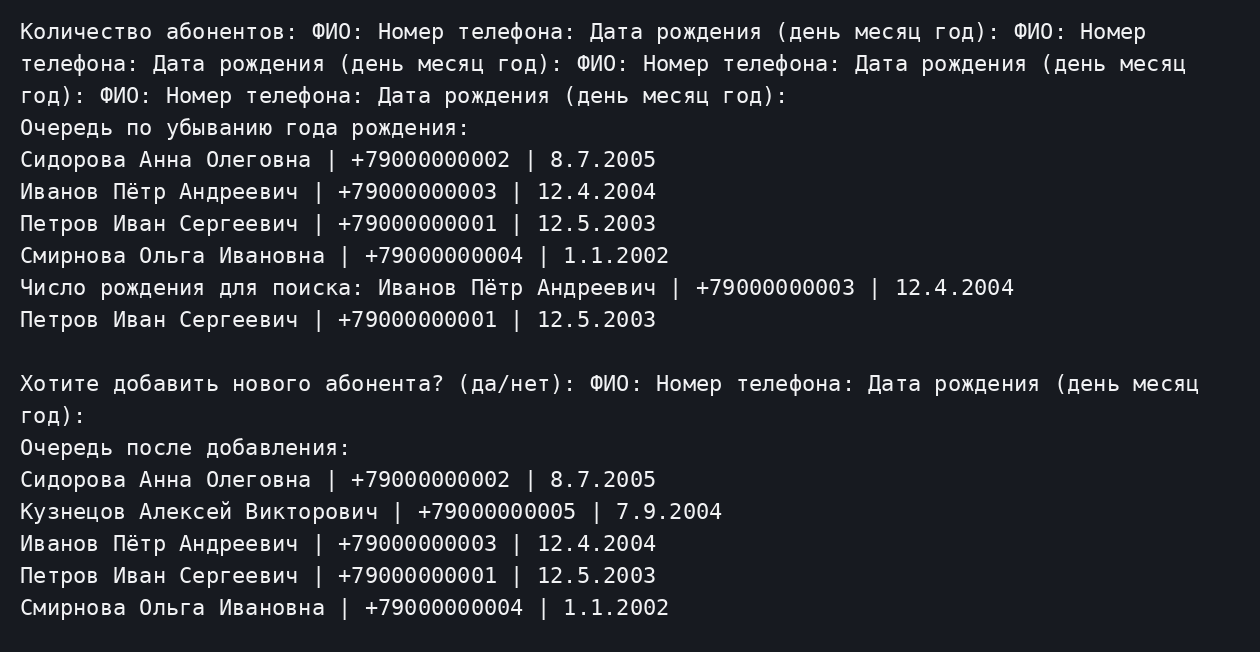
\includegraphics[width=\textwidth]{result.png}
\captionof{figure}{Вывод программы на контрольном примере}
\end{center}
\end{document}
